\documentclass[tikz,border=6pt]{standalone}
\usepackage{fontspec}
\setmainfont{Arial}
\usepackage{tikz}
\usetikzlibrary{arrows.meta,positioning,fit,backgrounds,shapes.geometric,calc}

% --- palette (matches scripts/figstyle.py) ---
\definecolor{titlegray}{HTML}{5F6B78}
\definecolor{ent}{HTML}{7B8794}
\definecolor{fo}{HTML}{5AA9C4}
\definecolor{ho}{HTML}{2E6B86}
\definecolor{sma}{HTML}{2E8AA6}
\definecolor{kg}{HTML}{E7B15A}
\definecolor{vio}{HTML}{9B86C4}
\definecolor{fillteal}{HTML}{E3EEF2}
\definecolor{filllav}{HTML}{ECE8F4}
\definecolor{fillamber}{HTML}{FBF0E2}
\definecolor{fillgrey}{HTML}{F1F3F5}
\definecolor{fillgreen}{HTML}{E6F0E6}

\begin{document}
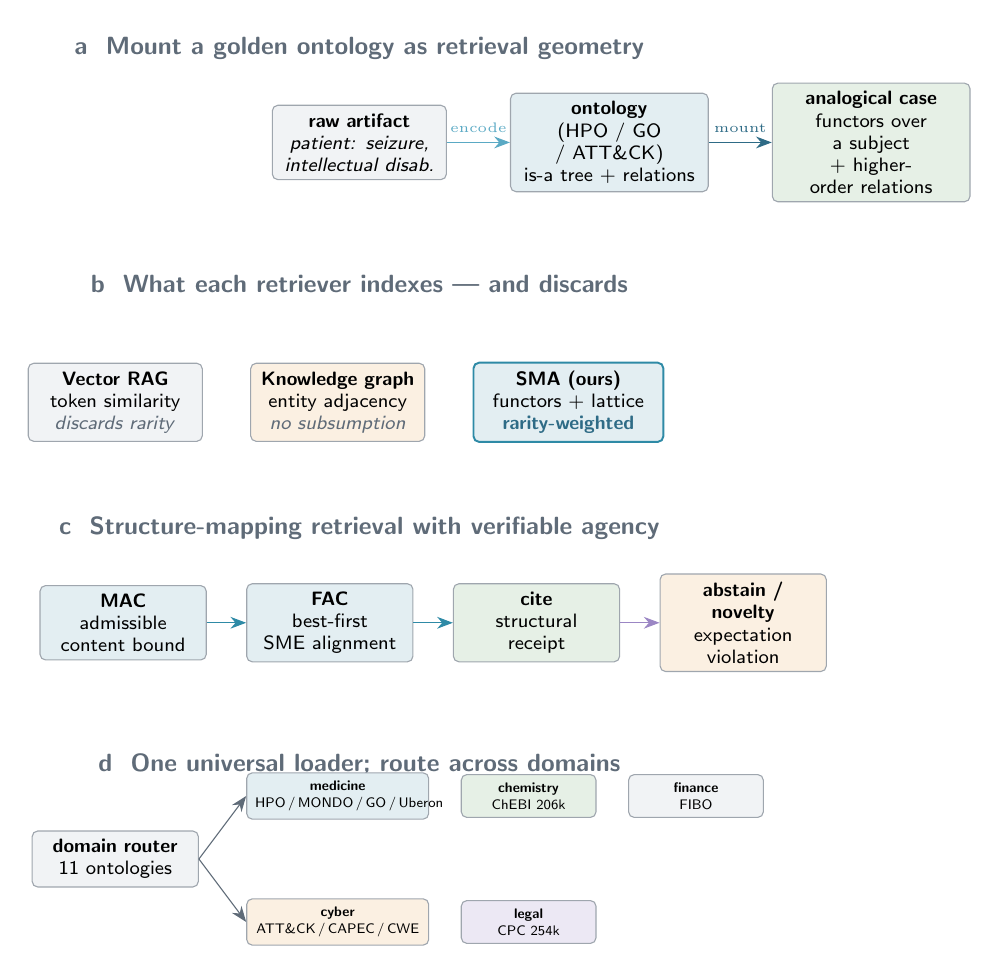
\begin{tikzpicture}[
  font=\sffamily\scriptsize,
  >={Stealth[length=2mm]},
  box/.style={rounded corners=2pt,draw=titlegray!60,line width=0.4pt,inner sep=3pt,align=center},
  node distance=4mm,
  panel/.style={titlegray,font=\sffamily\bfseries\small},
]

% ============ PANEL a: mount an ontology ============
\node[panel] (la) at (0,5.4) {a\ \ Mount a golden ontology as retrieval geometry};
\node[box,fill=fillgrey,text width=2.0cm] (raw) at (0,4.2)
  {\textbf{raw artifact}\\\textit{patient: seizure,}\\\textit{intellectual disab.}};
\node[box,fill=fillteal,text width=2.3cm,right=8mm of raw] (onto)
  {\textbf{ontology}\\(HPO / GO / ATT\&CK)\\is-a tree + relations};
\node[box,fill=fillgreen,text width=2.3cm,right=8mm of onto] (case)
  {\textbf{analogical case}\\functors over a subject\\+ higher-order relations};
\draw[->,fo] (raw) -- (onto) node[midway,above,font=\tiny]{encode};
\draw[->,ho] (onto) -- (case) node[midway,above,font=\tiny]{mount};

% ============ PANEL b: three retrieval geometries ============
\node[panel] (lb) at (0,2.4) {b\ \ What each retriever indexes --- and discards};
% vector RAG
\node[box,fill=fillgrey,text width=2.0cm] (rag) at (-3.1,0.9)
  {\textbf{Vector RAG}\\token similarity\\\textcolor{titlegray}{\textit{discards rarity}}};
% KG
\node[box,fill=fillamber,text width=2.0cm,right=6mm of rag] (kgb)
  {\textbf{Knowledge graph}\\entity adjacency\\\textcolor{titlegray}{\textit{no subsumption}}};
% SMA
\node[box,fill=fillteal,text width=2.2cm,right=6mm of kgb,draw=sma,line width=0.7pt] (smab)
  {\textbf{SMA (ours)}\\functors + lattice\\\textcolor{ho}{\textbf{rarity-weighted}}};

% ============ PANEL c: retrieve + verify ============
\node[panel] (lc) at (0,-0.7) {c\ \ Structure-mapping retrieval with verifiable agency};
\node[box,fill=fillteal,text width=1.9cm] (mac) at (-3.0,-1.9){\textbf{MAC}\\admissible\\content bound};
\node[box,fill=fillteal,text width=1.9cm,right=5mm of mac] (fac){\textbf{FAC}\\best-first\\SME alignment};
\node[box,fill=fillgreen,text width=1.9cm,right=5mm of fac] (cite){\textbf{cite}\\structural\\receipt};
\node[box,fill=fillamber,text width=1.9cm,right=5mm of cite] (nov){\textbf{abstain / novelty}\\expectation\\violation};
\draw[->,sma] (mac)--(fac); \draw[->,sma] (fac)--(cite); \draw[->,vio] (cite)--(nov);

% ============ PANEL d: registry + router ============
\node[panel] (ld) at (0,-3.7) {d\ \ One universal loader; route across domains};
\node[box,fill=fillgrey,text width=1.9cm] (router) at (-3.1,-4.9){\textbf{domain router}\\11 ontologies};
\node[box,fill=fillteal,text width=2.1cm,font=\sffamily\tiny,right=6mm of router,yshift=8mm] (med){\textbf{medicine}\\HPO\,/\,MONDO\,/\,GO\,/\,Uberon};
\node[box,fill=fillamber,text width=2.1cm,font=\sffamily\tiny,right=6mm of router,yshift=-8mm] (cyb){\textbf{cyber}\\ATT\&CK\,/\,CAPEC\,/\,CWE};
\node[box,fill=fillgreen,text width=1.5cm,font=\sffamily\tiny,right=4mm of med] (chem){\textbf{chemistry}\\ChEBI 206k};
\node[box,fill=filllav,text width=1.5cm,font=\sffamily\tiny,right=4mm of cyb] (leg){\textbf{legal}\\CPC 254k};
\node[box,fill=fillgrey,text width=1.5cm,font=\sffamily\tiny,right=4mm of chem] (fin){\textbf{finance}\\FIBO};
\draw[->,titlegray] (router.east)-- (med.west); \draw[->,titlegray] (router.east)-- (cyb.west);

\end{tikzpicture}
\end{document}
